\documentclass[12pt,a4paper]{article}
\usepackage[left = 35mm, right=35mm, top=20mm, bottom=44mm]{geometry} % To visualize margins
\usepackage[version=3]{mhchem} % Package for chemical equation typesetting
\usepackage{siunitx} % Provides the \SI{}{} and \si{} command for typesetting SI units
\usepackage{graphicx} % Required for the inclusion of images
\usepackage{mathptmx} % Times Roman font 
\usepackage{paralist} % For compactitem lists
\usepackage{color} % Color management options
\usepackage{listings} % To typeset source code
\usepackage{pdflscape} % Landscape pages
%\usepackage[acronym]{glossaries}
\usepackage{fancyhdr}
\usepackage[style=authoryear,backend=biber]{biblatex}
\addbibresource{bibliography.bib}
\usepackage{subcaption}
\usepackage{float}
\usepackage{textcomp}
\usepackage{acro}
\usepackage{longtable}
\usepackage[table]{xcolor}
\usepackage{array}
\usepackage{subcaption}
\usepackage{iftex}
\usepackage{soul}
\usepackage{tabularx}%this and one below for tables
\usepackage{booktabs}
\ifxetex
\usepackage[math-style=TeX, bold-style=TeX, ]{unicode-math}
\setmainfont{Times New Roman}
\setsansfont[Scale=MatchLowercase]{Arial}
\setmonofont[Scale=MatchLowercase]{Courier New}
\defaultfontfeatures{Ligatures=TeX}
\let\bm\symbfit
\else
\usepackage[utf8]{inputenc}%.................. Unicode file format
\usepackage{textcomp}%........................ Additional text symbols
\usepackage[T1]{fontenc}%..................... Type 1 outline fonts
\usepackage{bm}%.............................. Bold math fonts
\fi
\normalfont
\usepackage{sectsty}
\usepackage{enumitem}

\sectionfont{\fontsize{19}{18}\selectfont}
\subsectionfont{\fontsize{15}{16}\selectfont}
\subsubsectionfont{\fontsize{13}{14}\selectfont}
\newcommand\sumheading{%
	\rowcolor[gray]{.9}%
	\centering\arraybackslash%
	\bfseries\normalsize}
	
\geometry{
	a4paper,
	left=35mm,
	right=35mm,
	top=26mm,
	bottom=44mm
}
% Remove marginpar space (prevents visual extra right gutter)
\setlength{\marginparwidth}{0pt}
\setlength{\marginparsep}{0pt}
\setlength\parindent{0cm} % Set indentation for paragraphs
\setlength{\parskip}{0.5em}  % space between paragraphs
% To make floats, on float only pages, placed at top.
\makeatletter
\setlength{\@fptop}{0pt}
\setlength{\@fpbot}{0pt plus 1fil}
\makeatother

\DeclareAcronym{pgm}{
	short = PGM,
	long = Probabilistic Graphical Model,
	tag = abbrev
}

\DeclareAcronym{yolo}{
	short = YOLO,
	long  = You Only Look Once,
	tag   = abbrev
}

\DeclareAcronym{cv}{
	short = CV,
	long = Computer Vision,
	tag = abbrev
}

\DeclareAcronym{cnn}{
	short = CNN,
	long = Convolution Neural Network,
	tag = abbrev
}

\DeclareAcronym{rcnn}{
	short = R-CNN,
	long = Recurrent Convolution Neural Network,
	tag = abbrev
}
\DeclareAcronym{dl}{
	short = DL,
	long = Deep Learning,
	tag = abbrev
}
\DeclareAcronym{rv}{
	short = RV,
	long = Random Variable,
	tag = abbrev
}
\DeclareAcronym{bn}{
	short = BN,
	long = Bayesian Network,
	tag = abbrev
}
\DeclareAcronym{mn}{
	short = MN,
	long = Markov Network,
	tag = abbrev
}
\DeclareAcronym{cpd}{
	short = CPD,
	long = Conditional Probability Distribution,
	tag = abbrev
}
\DeclareAcronym{bp}{
	short = BP,
	long = Belief Propagation,
	tag = abbrev
}
\DeclareAcronym{bu}{
	short = BU,
	long = Belief Update,
	tag = abbrev
}
\DeclareAcronym{ipa}{
	short = IPA,
	long = Image Processing Algorithms,
	tag = abbrev

}
\DeclareAcronym{ml}{
	short = ML,
	long = Machine Learning,
	tag = abbrev
}
\DeclareAcronym{clg}{
	short = CLG,
	long = Conditional Linear Gaussian,
	tag = abbrev
}
\DeclareAcronym{ep}{
	short = EP,
	long = Expectation Propagation,
	tag = abbrev
}
\DeclareAcronym{adf}{
	short = ADF,
	long = Assumed Density Filtering,
	tag = abbrev
}
\DeclareAcronym{fps}{
	short = FPS,
	long = Frames Per Second,
	tag = abbrev
}
% Symbols
\DeclareAcronym{pa}{
	short = \ensuremath{P(A)},
	long  = Probability of event \(A\) occurring,
	sort  = pa,
	tag   = symbol
}

\DeclareAcronym{pagb}{
	short = \ensuremath{P(A \mid B)},
	long  = Conditional probability of event \(A\) given event \(B\),
	sort  = pab,
	tag   = symbol
}

\DeclareAcronym{pjoint}{
	short = \ensuremath{P(X_1, \dots, X_n)},
	long  = Joint probability distribution over variables \(X_1\) through \(X_n\),
	sort  = pjoint,
	tag   = symbol
}

\DeclareAcronym{px}{
	short = \ensuremath{p(x)},
	long  = Probability density function with respect to variable \(x\),
	sort  = px,
	tag   = symbol
}


\DeclareAcronym{pxgy}{
	short = \ensuremath{p(x \mid y)},
	long  = Conditional probability density of \(x\) given \(y\),
	sort  = pxy,
	tag   = symbol
}

\DeclareAcronym{muab}{
	short = \ensuremath{\mu_{a,b}},
	long  = Message from cluster \(a\) to cluster \(b\),
	sort  = muab,
	tag   = symbol
}

\DeclareAcronym{sum}{
	short = \ensuremath{\Sigma},
	long  = Summation operation,
	sort  = sigma,
	tag   = symbol
}

\DeclareAcronym{phi}{
	short = \ensuremath{\phi},
	long  = Potential or cluster,
	sort  = phi,
	tag   = symbol
}

\title{\textbf{Combining object tracking algorithms with probabilistic graphical models for accurate ball localization}}
	
\author{Alex Thorpe \textsc{}} % Author name
	
	\date{\today} % Date for the report
	
	\makeatletter
	\let\thetitle\@title
	\let\theauthor\@author
	\let\thedate\@date
	\makeatother

\renewcommand{\theequation}{\arabic{equation}}

\begin{document}
	\begin{titlepage}
	\centering
	
\includegraphics[scale = 1.5]{SU_logo_RGB-01.png}\\[1.0 cm]   % University Logo
	\textsc{\LARGE Mechatronic Project 478\\Final Report}\\[0.5 cm]               
	% Course Name
	\rule{0.9\textwidth}{0.2 mm} \\[0.4 cm]
	{ \huge \bfseries \thetitle }\\[0.4 cm]
	\rule{0.9\textwidth}{0.2 mm} \\[1.5 cm]
	
	\begin{minipage}{6.5cm}
		\begin{flushleft} \large
			\emph{Author:}\\
			\theauthor
		\end{flushleft}
	\end{minipage}~
	\begin{minipage}{6.5cm}
		\begin{flushright} \large
			\emph{Student Number:} \\
			{25934171}
		\end{flushright}
	\end{minipage}\\[2 cm]
	{\large \thedate}\\[1 cm]
	{\large Supervisor: Dr. C. E. Van Daalen}\\[1 cm]
	\vfill
	
\end{titlepage}

\pagenumbering{roman}
\setcounter{page}{1}
\fancyfoot[C]{\thepage}
        
%\section*{Acknowledgments}
%\pagenumbering{roman}
%\addcontentsline{toc}{section}{Acknowledgments}
%\newpage
\section*{Plagiarism Declaration}
\addcontentsline{toc}{section}{Plagiarism Declaration}
I have read and understand the Stellenbosch University Policy on Plagiarism and the definitions of plagiarism and self-plagiarism contained in the Policy [Plagiarism: The use of the ideas or material of others without acknowledgement, or the re-use of one's own previously evaluated or published material without acknowledgement or indication thereof (self-plagiarism or text-\-re\-cyc\-ling)].

I also understand that direct translations are plagiarism, unless accompanied by an appropriate acknowledgement of the source. I also know that verbatim copy that has not been explicitly indicated as such, is plagiarism.

I know that plagiarism is a punishable offence and may be referred to the University's Central Disciplinary Committee (CDC) who has the authority to expel me for such an offence.

I know that plagiarism is harmful for the academic environment and that it has a negative impact on any profession.

Accordingly all quotations and contributions from any source whatsoever (including the internet) have been cited fully (acknowledged); further, all verbatim copies have been expressly indicated as such (e.g. through quotation marks) and the sources are cited fully.

I declare that, except where a source has been cited, the work contained in this assignment is my own work and that I have not previously (in its entirety or in part) submitted it for grading in this module/assignment or another module/assignment.
I declare that have not allowed, and will not allow, anyone to use my work (in paper, graphics, electronic, verbal or any other format) with the intention of passing it off as his/her own work.

I know that a mark of zero may be awarded to assignments with plagiarism and also that no opportunity be given to submit an improved assignment.
\vspace{1cm}
\begin{table}[ht]
	\begin{center}
		\begin{tabular*}{15.5cm}{@{\extracolsep{\fill}}lll}
			%		\begin{tabular}{l l l}
				
\includegraphics[width=2cm]{Signature.jpeg} & & 25934171\\
				\makebox[8cm]{\hrulefill} & & \makebox[6cm]{\hrulefill}\\
				Signature & & Student number\\[1cm]
				\theauthor & & \thedate\\
				\makebox[8cm]{\hrulefill} & & \makebox[6cm]{\hrulefill}\\ 
				Initials and surname & & Date \\
			\end{tabular*}
		\end{center}
	\end{table}
	
	\newpage

\section*{Executive Summary}
\addcontentsline{toc}{section}{Executive Summary}
\noindent
\begin{longtable}{|p{\dimexpr \linewidth-2\tabcolsep-2\arrayrulewidth}|}
	\hline%------------------------------------------------------------
	\sumheading  Title of Project \\
	\hline%------------------------------------------------------------
	Combining Object Tracking Algorithms with Probabilistic Graphical Models for Accurate Ball Localization \\[1ex]
	
	\hline%------------------------------------------------------------
	\sumheading  Objectives \\
	\hline%------------------------------------------------------------
	This project aims to estimate a ball’s position in real time using standard video footage. Multiple object tracking algorithms will be applied, and their outputs fused using a probabilistic graphical model (PGM) to enhance accuracy, robustness, and responsiveness. The final goal is to evaluate the PGM-based fusion model against individual trackers. \\[1ex]
	
	\hline%------------------------------------------------------------
	\sumheading  What is current practice and what are its limitations? \\
	\hline%------------------------------------------------------------
	Hawk-Eye and Tracab are industry leaders in ball tracking and sports officiating. Hawk-Eye supports over 20 sports with real-time tracking and visualization, while Tracab focuses on football, analyzing player movement and ball trajectory \parencite{hawkeye2024, tracab2024}. Despite their accuracy, both systems require complex, expensive multi-camera setups and proprietary infrastructure, limiting their use in smaller-scale, research, or open-source applications. \\[1ex]
	
	\hline%------------------------------------------------------------
	\sumheading  What is new in this project? \\
	\hline%------------------------------------------------------------
	This project introduces an accurate, low-complexity ball tracking system that requires minimal camera infrastructure, making it accessible for research, amateur sports, and low-budget environments.\\[1ex]
	
	\hline%------------------------------------------------------------
	\sumheading  If the project is successful, how will it make a difference? \\
	\hline%------------------------------------------------------------
	If successful, this project could enhance decision-making across various sports by accurately determining ball location in real time — such as confirming goals or out-of-bounds events — making advanced tracking more accessible beyond elite-level systems. \\[1ex]
	
	\hline%------------------------------------------------------------
	\sumheading  What are the risks to the project being a success? Why is it expected to be successful? \\
	\hline%------------------------------------------------------------
	A key risk is that the system may not match the efficiency or accuracy of existing commercial trackers, limiting its ability to fully replace them. However, by studying and building on established tracking methods, this project is expected to deliver a more lightweight and accessible alternative — one that balances performance with lower complexity and cost. \\[1ex]
	
	\hline%------------------------------------------------------------
	\sumheading  What contributions have/will other students made/make? \\
	\hline%------------------------------------------------------------
	N/A \\[1ex]
	
	\hline%------------------------------------------------------------
	\sumheading  Which aspects of the project will carry on after completion and why? \\
	\hline%------------------------------------------------------------
	After completion, the project could be extended by incorporating sport-specific rules, enabling the system to automatically detect rule violations such as offside positions, fouls, or out-of-bounds events. This would build on the core tracking functionality and move the system toward real-time decision support and automated officiating. \\[1ex]
	
	\hline%------------------------------------------------------------
	\sumheading  What arrangements have been/will be made to expedite continuation? \\
	\hline%------------------------------------------------------------
	All components of the project will be thoroughly documented, with clear definitions of the system architecture, algorithms, and data handling. This will ensure the project can be easily continued by future students or refined further for potential commercialization.\\[1ex]
	
	\hline%------------------------------------------------------------
\end{longtable}
\newpage

\section*{Evaluation of ECSA Exit Level Outcomes}
\addcontentsline{toc}{section}{Evaluation of ECSA Exit Level Outcomes}
\renewcommand{\arraystretch}{3} % More vertical spacing
\rowcolors{2}{gray!10}{white}     % Alternating row colors

\begin{longtable}{|p{0.6\linewidth}|p{0.35\linewidth}|}
\hline
\rowcolor{gray!30}
\multicolumn{2}{|c|}{\textbf{ECSA Outcomes Assessed in this Module}} \\
\hline
\textbf{ECSA Outcome} & \textbf{Addressed} \\
\hline
\textbf{GA 1. Problem solving:} Demonstrate competence to identify, assess, formulate and solve convergent and divergent engineering problems creatively and innovatively. & Throughout the literature review process and figuring out the algorithms. \\
\hline
\textbf{GA 2. Application of scientific and engineering knowledge:} Demonstrate competence to apply knowledge of mathematics, basic science and engineering sciences from first principles to solve engineering problems. & During the experimentation and testing portion of the project and when applying the algorithms. \\
\hline
\textbf{GA 3. Engineering Design:} Demonstrate competence to perform creative, procedural and non-procedural design and synthesis of components, systems, engineering works, products or processes. & During the concept design and algorithm decision. \\
\hline
\textbf{GA 5. Engineering methods, skills and tools, including Information Technology:} Demonstrate competence to use appropriate engineering methods, skills and tools, including those based on information technology. & Throughout the project the use of different coding methods will be used and learning new skills such as PGMs. \\
\hline
\textbf{GA 6. Professional and technical communication:} Demonstrate competence to communicate effectively, both orally and in writing, with engineering audiences and the community at large. & Project Proposal; Progress Report; Preliminary Draft; Final Report; Oral Presentation; Project Poster. \\
\hline
\textbf{GA 8. Individual, Team and Multidisciplinary Working:} Demonstrate competence to work effectively as an individual, in teams and in multidisciplinary environments. & This project shows individual work very clearly. \\
\hline
\textbf{GA 9. Independent Learning Ability:} Demonstrate competence to engage in independent learning through well-developed learning skills. & Will have to self-learn many different complex topics. \\
\hline
\end{longtable}
\newpage

\tableofcontents
\newpage
\listoffigures
\newpage
\listoftables
\newpage
\printacronyms[include = abbrev, name = {List of Abbreviations}]
\newpage
\printacronyms[include=symbol, name = {List of Symbols}]
\newpage

\pagenumbering{arabic}
\setcounter{page}{1}
\section{Introduction}
The growing importance of data-driven decision-making in sports has accelerated the adoption of advanced technologies such as \acl{ml} (\acs{ml}), computer vision, and real-time analytics. In particular, ball tracking has become a critical component in modern sports for enhancing player performance analysis, enabling data-supported officiating, and facilitating targeted training interventions. High-profile systems such as Hawk-Eye and TRACAB have become industry standards, Hawk-Eye being widely used for adjudication in tennis and cricket \parencite{hawkeye2024}, while TRACAB supports tactical and performance analysis in football and other team sports \parencite{tracab2024}.

Despite their effectiveness, these systems depend on dense camera arrays and high-performance computing infrastructure installed around stadiums, resulting in high operational costs. Consequently, their deployment is largely limited to professional leagues and elite-level clubs. This creates a gap for smaller leagues, grassroots sports organizations, and researchers who require tracking tools but lack access to such costly resources.

This project investigates a low-cost, accessible solution for real-time ball tracking using pre-recorded video footage sourced from online platforms. By implementing and comparing multiple lightweight tracking algorithms—including classical computer vision techniques and pre-trained object detectors such as \acs{yolo}—the project aims to develop a robust pipeline capable of estimating the ball's position. A key innovation in the proposed framework is the fusion of uncertain outputs from multiple \acl{ipa} (\acs{ipa}) using a Probabilistic Graphical Model (PGM), which enables robust inference even in the presence of noise and partial information \parencite{koller2009pgm}. This probabilistic fusion strategy helps mitigate the limitations of individual trackers and reduces overall tracking errors, particularly in challenging conditions such as occlusion and motion blur.

The objective is to develop a cost-effective and computationally efficient tracking system that can run on consumer-grade hardware without compromising significantly on accuracy. This contributes to the democratization of sports analytics, opening the door to broader adoption in non-professional environments such as university clubs, school competitions, and community sports settings.

This research is conducted by Mr. A.H. Thorpe as part of the Mechatronic Project 478/488 under the supervision of Dr. Corne Van Daalen. It aligns with the graduate attributes prescribed by the Engineering Council of South Africa (ECSA).

\subsection{Motivation}
In many sports, decisions made by officials are often prone to error because they rely heavily on human judgment. These errors can accumulate, with some leagues averaging up to five officiating mistakes per match \parencite{ref_officiating_error}. For example, in the Premier League, referees still rely on manually drawing lines on video footage to determine ball position for offside or goal-line decisions \parencite{premier_league_offside}. While this method can be effective, it remains susceptible to inaccuracies caused by varying camera angles and inherent human limitations. An accurate, real-time ball tracking system could significantly improve decision-making by providing objective and precise positional data, reducing inconsistencies during match officiating \parencite{hawk_eye_system}.

Beyond officiating, precise ball tracking also offers substantial benefits in player training and performance analysis. By capturing various aspects of both player movement and ball dynamics, coaches and athletes can gain deeper insights into performance metrics, enabling targeted improvements in technique, decision-making, and strategy. Such data-driven feedback has been shown to enhance skill development and game understanding across multiple sports disciplines \parencite{tracking_training_benefits}.

In addition to these high-level benefits, many smaller clubs, schools, and amateur leagues lack the resources to implement advanced commercial tracking systems such as Hawk-Eye or TRACAB. These systems require high-performance cameras and computing infrastructure, making them inaccessible to most grassroots or academic environments. There is a clear need for a low-cost, computationally efficient alternative that can run on widely available consumer-grade hardware.

To address this gap, the project proposes a lightweight video-based tracking framework capable of estimating the ball’s position in three-dimensional space using multiple complementary detection techniques. By combining the strengths of different methods, the system aims to deliver reliable tracking performance even under challenging conditions such as occlusion or motion blur.

\subsection{Objectives}
The objective of this project is to develop a model that can accurately and reliably estimate the position of a ball in real time using pre-recorded video footage. This will be achieved through the fusion of multiple \acs{ipa}, each capable of independently detecting the ball's position. The outputs of these algorithms will be combined using a \acs{pgm} to improve robustness and reduce the estimation error in position. The following objectives define the scope of this project:

\begin{enumerate}
	\item Develop and implement multiple \acs{ipa} to estimate the ball’s position from video footage.
	\item Design a \acs{pgm}-based fusion method to combine the outputs of individual algorithms, improving tracking accuracy and reducing errors from isolated failures.
	\item Evaluate and optimize the system to use the minimal number of algorithms required while maintaining acceptable performance.
	\item Compare the final model’s performance against each individual algorithm in terms of accuracy, robustness, and computational efficiency.
\end{enumerate}

\subsection{Report Overview}
This section outlines each section that will be discussed in this report. The idea gets formed and the objectives set in Chapter 1. Chapter 2 focuses on the background and literature of the project where core concepts get formed from existing work. From there the Model Design takes place in Chapter 3, this is where the requirements of the \acs{ipa}s and \acs{pgm}s are set. Chapter 4 will then go into the implementation of the \acs{ipa}s and \acs{pgm} and how the final Algorithms are choosen. Chapter 5 then goes into Experimentation and how the various parameters for the \acs{ipa} and \acs{pgm} were selected. Finally the last chapter will cover the conclusion of the report.


\newpage
\section{Background and Literature Review}
Object tracking is a task that dates back to the earliest days of human civilization, from following animal tracks to observing celestial bodies for navigation. As technology has advanced, computers have become a key tool in tracking objects with high precision. One of the most common examples in modern life is the Global Positioning System (GPS), which allows users to determine their position anywhere on Earth \parencite{challa2011fundamentals}.

A major industry that relies heavily on object tracking is sports. Companies such as Hawk-Eye and TRACAB are global leaders in this domain, with Hawk-Eye specializing in officiating decisions and TRACAB focusing on performance analysis and training \parencite{tracab2024,hawkeye2024}. Accurate tracking in sports benefits a wide range of stakeholders — from fans and broadcasters to coaches, players, and officials \parencite{labayen2014accurate}. Given that sports are governed by clear rules and boundaries, it is natural that computer-aided systems are increasingly being used to enhance decision-making on and off the field.

Despite its advantages, ball tracking in sports presents numerous challenges. Balls tend to be small, fast-moving objects, often affected by motion blur and frequent occlusion in video footage. These issues can severely limit the performance of traditional image processing techniques. Furthermore, the nature of the tracking problem can vary significantly between sports. For instance, in table tennis, the ball exhibits highly nonlinear and non-periodic motion, making it particularly difficult to track reliably \parencite{kamble2019ball}.

Because of these challenges, no single tracking algorithm can perform robustly in all scenarios. Each technique has its own weaknesses depending on the scene, motion, and visual obstructions. This motivates the use of \acl{pgm}s, which provide a principled framework for combining uncertain outputs from multiple algorithms \parencite{koller2009pgm}. \acs{pgm}s allow relationships between multiple random variables to be explicitly modeled, making them particularly useful for data fusion and robust inference under uncertainty.

This section provides a review of the core technical concepts and prior work relevant to this project. It includes discussions on existing commercial tracking systems, \acl{cv} techniques for tracking, \acs{ipa}, \acs{pgm}s and, identifies the current gaps in the literature that this project aims to address.

\subsection{Existing Commercial Tracking systems}
As mentioned in the introduction, two of the leading commercial solutions for ball tracking in sports are Hawk-Eye and TRACAB. Hawk-Eye operates using an array of high-speed cameras positioned around the stadium to capture the ball's trajectory in real time with sub-millimetre accuracy \parencite{tennisnerd2024hawk-eye}. This system, while highly accurate, is prohibitively expensive for widespread use. Installation costs range between R1 million and R1.25 million per court (approximately \$55,000–\$70,000 USD), making it inaccessible to amateur clubs and individuals \parencite{wong2016lowcost}. In addition to its cost, Hawk-Eye requires complex infrastructure, including camera placements two to three stories above the field, which adds to the installation difficulty and venue constraints.

TRACAB, another global leader, combines camera-based tracking with sensor-based solutions. The system includes multiple high-speed cameras—often sourced from Hawk-Eye—alongside a sensor chip embedded in the ball, developed by the German company Cairos Technology AG \parencite{wipo2023goalline}. TRACAB is commonly used for both training applications and goal-line decision-making. However, its cost is even higher, with installation reported at around R5 million (approx. \$270,000 USD) and an additional R70,000 (approx. \$3,800 USD) per game to operate the system \parencite{wiebe2013mls}.

While these high-end systems are effective, they are far beyond the reach of most local sports clubs, schools, and individual athletes. More affordable alternatives are emerging, such as XBotGo, which offers a ball-tracking system for a once-off cost of approximately R6,300 (about \$340 USD) \parencite{xbotgo2024chameleon}. Although this represents a more accessible option, it still requires the user to provide their own compatible camera equipment, which contributes to the total cost. Additionally, shipping limitations may restrict access to certain regions, particularly in developing countries.

\subsection{Computer Vision techniques for tracking}
\acl{cv} is used when significant information is needed to be extracted from images \parencite{stockmanComputerVision}. In terms of tracking objects this is vital, as this opens the door to be able to extract vital information of where the object is located. The foundation of object tracking is object detection, which is identifying an object of interest in an image. Wheres object tracking evolved into is being able to "see" the motion of the object as it moves through the frames of a video\parencite{zhao2015overview}. Object tracking doesn't come without its challenges with the most common being occlusion, illumination variation, and fast motion\parencite{soleimanitaleb2019object}.

\subsubsection{Traditional Tracking and Detecting methods}
There are many different methods that lead to how \acs{cv} was used for tracking but most of them are based on foundational mathematics and statistics. 

One such example uses recursive Bayesian logic formulated and derived from the Bayesian probabilistic framework. Examples of algorithms traditionally found are the Kalman filter, extended Kalman filter, unscented Kalman filter, point mass filter, and particle filter. These algorithms were developed to find a resolution to generic estimation and filtering problems \parencite{challa2011fundamentals}.

An example based on using mathematical models for detection and tracking is from a study done in 2013 that proposed an algorithm based on integrating the mechanisms of the Human Visual System (HVS) where it detected and tracked infrared dim and a small target. The method is based on 4 steps, firstly a multi-scale Difference of Gaussians, which is a method of detecting features of different scales, which is then placed in feature maps at different scales, the next step was to add a Gaussian window to this map at a location near the object, the penultimate step was to normalize the image and decide on the location of the object in this frame and if this is the final step the algorithm stops. However if there is another frame it estimates the location on the next frame via a Proportional-Integral-Derivative algorithm and goes back to step 1\parencite{Mirzaei2016, dong2014infrared}.

These both provide an idea of what is traditionally done in terms of tracking and detecting objects through \acs{cv}.

\subsubsection{Modern Deep Learning-Based Tracking}
As technology in software and hardware advanced so did the methods in which tracking and detecting was done, \acl{cnn} based on \acl{dl} technology\parencite{pal2021deep}, which is a relatively recent breakthrough in \acs{cv} and how tracking is done from video footage.

\acs{cnn}s are used to identify features in which they are used to localize and classify the objects within the frames\parencite{pal2021deep}, these make it a very powerful tool for tracking and detecting objects. There are two methods, being discriminative and generative. The discriminative method focuses on binary classification, often called \acs{cnn}-C, which distinguishes an object from its background. The Generative method, often called \acs{cnn}-M focuses on learning a robust similarity function, which aims to find a match to the object template from a specified region\parencite{li2018deep}.

There are a few common modern approaches to object detection, one being the use of \acs{cnn} as described in the previous paragraph, Transformer based approaches, Vision Language models and lastly Hybrid models such as RetinaMask and EfficientDet\parencite{sapkota2025rf}. A benefit of \acs{yolo} is that it has been trained on the COCO dataset to be able to detect sports balls as well as that \acs{yolo} has a small model size and fast calculation speed. 

\subsection{Image Processing Algorithms}
This section discusses how \acs{ipa} can be used to extract relevant raw data for the \acs{pgm}s. \acl{ipa} (\acs{ipa}) is a term that can be used in equivalence to \acs{cv} as in many cases \acs{ipa} simulates human vision \parencite{pitas2000}. 

\acs{ipa} can be broken down into 3 distinct categories, Low-Level, Intermediate level, and High-level vision algorithms. The low-level vision focuses on the most basic operations applied to raw pixels, the goal is to improve the image quality or extract very simple features. The intermediate level vision takes this cleaned low-level vision image and organizes these pixels into meaningful structures, this helps bridge the gap between pixel-level data and understanding of the objects in the image. Finally the high-level vision, is where \acl{ml} (\acs{ml}) comes into play and allows for object recognition \parencite{pitas2000}.

\subsubsection{Low-Level Vision}
As stated before, low-level vision refers to the basic pixel-level processing that prepares raw images for higher-level interpretations \parencite{ji2013_3dvision_intro}. In order to accomplish this various techniques can be applied, these enhance the image without altering underlying information within the image. The techniques that can be used are Edge Detection, this is where the operation identifies points on the image where brightness changes sharply, Filtering, which enhances certain aspects of an image, and finally Thresholding, which converts grayscaled images into binary images based on a threshold value \parencite{metaeye} by mapping intensity values above or below a threshold into distinct classes (such as the background and foreground). In practice this is commonly used in pre-processing video frames to enable more robust object detection and tracking.

\subsubsection{Intermediate Level Vision}
This level builds on the processing performed in low-level vision by assembling coherent objects and motion patterns. As discussed above this level bridges the gap between low-level and high-level visions \parencite{metaeye}. Similar to Low-level vision, several techniques are commonly used at the intermediate level. These include segmentation, which divides the image into various segments or regions that share similar attributes (For example the watershed algorithms or k-means clustering), Object detection which identifies and localizes objects within each frame and finally Optical flow which estimates the motion between two consecutive frames \parencite{metaeye}. Together all of these help to have a basic level of detection within the videos, such as tracking of a ball on the field. The final level being High-level vision is when classification of the objects come in, as this isn't in the scope of this project a further discussion is not needed.

\subsubsection{OpenCV}
OpenCV is an Open Source Computer Vision library for image and video analysis and was developed by Intel over two decades ago. Originally written in C++/C but now has wrappers for Python, Java or Matlab \parencite{culjak2012opencv}. The library possesses various techniques for Low-level vision, intermediate level vision and High-level vision \parencite{mohamad2015opencv}. Key functioning included are Threshold, Filtering, Finding edges, segmentation, background subtraction, and various other functions that can be applied to various different \acs{ipa} \parencite{marengoni2011opencv}. 

\subsubsection{OpenCV Functions for Low- and Intermediate-Level Vision}
This subsection provides a detailed breakdown of the low-level and intermediate-level vision functions available in OpenCV, which are relevant for image processing algorithms used in ball tracking. These functions are implemented in the library and can be accessed via Python bindings, as utilized in this project.

\paragraph{Low-Level Vision}
\mbox{}\\
As discussed previously low-level vision focuses on basic pixel-level processing that prepares videos or images for higher-level interpretations. The relevant functions available in OpenCV are summarized in Table~\ref{tab:lowlevel}.

\setcounter{table}{0}
\begin{longtable}{@{}l p{0.7\textwidth}@{}}
	\caption{Low-Level Vision Functions from OpenCV}
	\label{tab:lowlevel} \\
	\toprule
	\textbf{Operation} & \textbf{Description} \\
	\midrule
	\endfirsthead
	\toprule
	\textbf{Operation} & \textbf{Description} \\
	\midrule
	\endhead
	Thresholding & Converts grayscaled images into binary images based on a threshold value, this is useful for separating the object from the background. Can use functions like \texttt{cv2.threshold()} (applies a fixed threshold to pixel intensities for binary segmentation) \parencite{opencv_threshold} and \texttt{cv2.inRange()} (checks if the pixel values fall within a specified ranges for color-based masking) \parencite{opencv_inrange}. \\
	
	Filtering & Enhances certain aspects of an image, such as smoothing or sharpening, which in turn helps improve ball visibility. Can use functions like \texttt{cv2.medianBlur()} (replaces each pixel with the median intensity of neighboring pixels to reduce noise) \parencite{opencv_median} and \texttt{cv2.GaussianBlur()} (applies Gaussian smoothing, which blurs the image by averaging nearby pixels with weights that decrease with distance from the center, effectively reducing high-frequency noise while preserving edges better than uniform averaging) \parencite{opencv_gaussian}. \\
	
	Frame differencing & Computes the absolute difference between consecutive frames to detect motion. Can use \texttt{cv2.absdiff()} (calculates pixel-wise absolute difference for motion detection) \parencite{szeliski2010computer}. \\
	
	Finding edges & Identifies points where brightness changes sharply, which can help outline the ball against the court or field. Can use functions like \texttt{cv2.Canny()} (multi-stage edge detection which uses gradients and hysteresis thresholding) \parencite{opencv_canny} and \texttt{cv2.Sobel()} (computes image gradients for edge detection in horizontal or vertical directions) \parencite{opencv_sobel}. \\
	
	Color space conversion & Transforms images between different color spaces, which can enhance color-based segmentation of the ball. Can use \texttt{cv2.cvtColor()} (changes color representation, for example going from BGR to HSV for better color separation) \parencite{opencv_color}. \\
	
	Morphological operations & Techniques like dilation and erosion that refine binary images by removing noise and closing gaps in detected objects. Can use functions like \texttt{cv2.dilate()} (expands bright regions in binary images using a structuring element) \parencite{opencv_dilate}, \texttt{cv2.erode()} (shrinks bright regions to remove small noise) \parencite{opencv_erode}, and \texttt{cv2.morphologyEx()} (applies advanced operations like opening or closing for shape refinement) \parencite{opencv_morphologyex}. \\
	\bottomrule
\end{longtable}

\paragraph{Intermediate-Level Vision}
\mbox{}\\
Building on low-level processing, intermediate-level vision assembles coherent objects and motion patterns. The relevant functions available in OpenCV are summarized in Table~\ref{tab:intermediate}.

\begin{longtable}{@{}l p{0.7\textwidth}@{}}
	\caption{Intermediate-Level Vision Functions from OpenCV}
	\label{tab:intermediate} \\
	\toprule
	\textbf{Operation} & \textbf{Description} \\
	\midrule
	\endfirsthead
	\toprule
	\textbf{Operation} & \textbf{Description} \\
	\midrule
	\endhead
	Segmentation & Divides the image into segments or regions that share similar attributes, this helps isolate the ball. Can use functions like \texttt{cv2.findContours()} (detects contours in binary images for shape analysis) \parencite{opencv_contours}, \texttt{cv2.connectedComponents()} (labels connected regions in binary images for segmentation) \parencite{opencv_connected}, and \texttt{cv2.HoughCircles()} (detects circular shapes for ball-like object segmentation) \parencite{opencv_hough}. \\
	
	Object detection & Identifies and localizes objects within each frame, this is crucial for tracking the ball. Can use shape-based filtering with \texttt{cv2.findContours()} (detects contours for shape analysis) \parencite{opencv_contours}, \texttt{cv2.convexHull()} (computes convex hull for solidity) \parencite{opencv_convex}, and \texttt{cv2.arcLength()} (calculates perimeter for circularity) \parencite{opencv_arclength} to filter ball-like objects based on properties like aspect ratio, circularity, and solidity. \\
	
	Background subtraction & Separates moving foreground objects from the static background, useful for isolating the ball in video frames. Can use \texttt{cv2.createBackgroundSubtractorMOG2()} (creates a MOG2 background subtractor for motion detection) \parencite{opencv_bgsub}. \\
	
	Optical flow & Estimates motion between two consecutive frames, useful for predicting ball movement. Can use functions like \texttt{cv2.calcOpticalFlowFarneback()} (dense optical flow estimation using polynomial expansion) \parencite{opencv_farneback} and \texttt{cv2.calcOpticalFlowPyrLK()} (sparse optical flow using the Lucas-Kanade method) \parencite{opencv_pylk}. \\
	\bottomrule
\end{longtable}
	
\subsection{\acl{pgm}s}
\acl{pgm}s (\acs{pgm}s) offer a powerful framework for representing and reasoning about probabilistic relationships, allowing computers to answer complex questions under uncertainty. They are widely used across various applications, including speech recognition, image segmentation, disease outbreak modeling, and \acs{cv}, which is the primary focus of this project \parencite{koller2009pgm}. \acs{pgm}s combine probability theory and graph theory to create structured and interpretable models of complex distributions, and they scale effectively to high-dimensional problems. The structure and concepts throughout these following sub sections are based primarily on the foundational work presented by Koller and Friedman\parencite{koller2009pgm} as well as the courses presented by Daphne Koller on Coursera \parencite{kollerVideoGen1, kollerVideoGen2}.

This section explores the key concepts of \acs{pgm}s that are directly relevant to the object tracking approach developed in this project. It begins with a discussion on modeling, introducing the way graphical models are constructed and how probabilistic dependencies are encoded within them. Following that, the section discusses inference, describing how the various nodes in the model interact and how information is propagated throughout the graph to produce a coherent estimate. It then examines Gaussian factors, explaining how Gaussian distributions are used to represent uncertainty and how these distributions are applied to the outputs of image processing algorithms. Finally, it concludes by demonstrating how this probabilistic output is used for object tracking, and how it contributes to a more reliable and interpretable tracking system.

\subsubsection{Modeling}
Models are declarative representations of our understanding of the world. They take in input data, apply structured reasoning, often through algorithms, and produce output that is relevant to the user’s task. In the context of \acs{pgm}s, the modeling is done through probabilistic reasoning, which is essential for managing uncertainty.

When creating a model in the context of \acs{pgm}s, three main steps are typically followed. First, the \acl{rv}s (\acs{rv}) involved in the process are identified.

Next, a graphical model is constructed by selecting a representation suited to the problem. There are two main types of graphical models used in \acs{pgm}s: \acl{bn}s (\acs{bn}s), which are directed, and \acl{mn}s (\acs{mn}s), which are undirected. Examples of both are shown in Figure~\ref{fig:graph_networks}.

 \begin{figure}[htbp]
 	\centering
 	\begin{subfigure}[b]{0.45\textwidth}
 		\centering
 		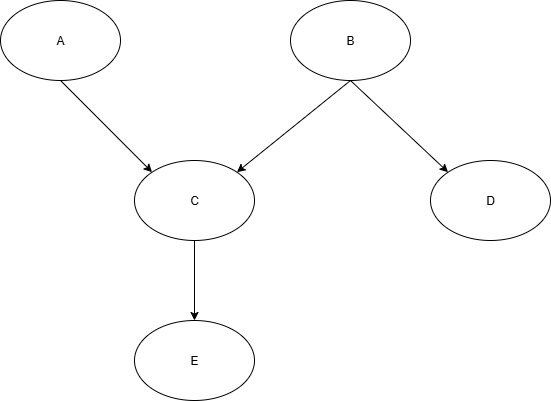
\includegraphics[width=\textwidth]{B_Network_Example.jpg}
 		\caption{Example of \acl{bn}}
 		\label{fig:bayesian_network}
 	\end{subfigure}
 	\hfill
 	\begin{subfigure}[b]{0.35\textwidth}
 		\centering
 		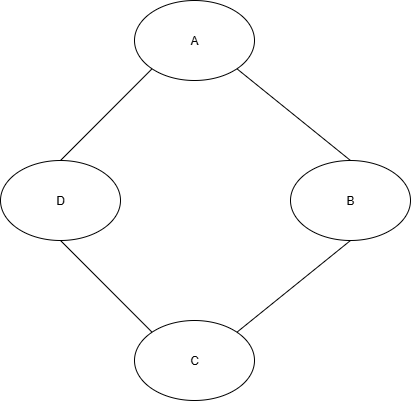
\includegraphics[width=\textwidth]{M_Network_Example.png}
 		\caption{Example of \acl{mn}}
 		\label{fig:markov_network}
 	\end{subfigure}
 	\caption{Examples of graphical models}
 	\label{fig:graph_networks}
 \end{figure}

In Figure~\ref{fig:bayesian_network}, the \acs{bn} is represented as a directed graph, where edges have arrows indicating conditional dependencies between random variables. A node with outgoing arrows is referred to as a parent, while nodes receiving those arrows are its children. For example, the arrow from node A to node C signifies that “C depends directly on A,” or equivalently, “A influences C.”

By contrast, the \acs{mn} in Figure~\ref{fig:markov_network} is undirected, with edges lacking any direction. This reflects symmetric dependencies: neither node is assumed to influence the other in a causal sense. In this case, the undirected edge between A and B indicates that “A and B are directly dependent,” without implying a specific direction of influence.

Finally, the last step is to define the factors required by the graph. For a \acs{bn}, each factor corresponds to a \acl{cpd} (\acs{cpd}), a conditional probability (\acs{pagb}) distribution for a variable given its parents. If a node has no parents, its factor is simply a marginal distribution \acs{pa}. For example, in the \acs{bn} from Figure~\ref{fig:bayesian_network}, the associated distributions are:

\begin{equation}P(A),  P(B),  P(C|A,B),  P(D|B),  P(E|C)\end{equation}

These are combined into one joint distribution (\acs{pjoint}) using the chain rule:

\begin{equation}P(A,B,C,D,E) = P(A).P(B).P(C|A,B).P(D|B).P(E|C)\end{equation}

This joint distribution can then be used like any other multivariate distribution.

While this approach is manageable for small networks, it becomes computationally expensive for larger ones. This is where inference comes in. The next section discusses how inference methods, particularly belief propagation, enable efficient probabilistic queries without explicitly computing full joint distributions.

\subsubsection{Inference}
Inference is the process of calculating probabilities of \acs{rv}s of interest given partial information. In practice, this means calculating the probability distribution of one \acs{rv} conditioned on observed evidence from other \acs{rv}s. This is very useful as in the real world not every \acs{rv} is observed, therefore the use of inference provides reason for unobserved \acs{rv}s.

All further explanations will be explained for \acs{bn} because they can be encoded into a \acs{mn}. This conversion from \acs{bn} to \acs{mn} involves removing the directional edges as well as making the inference more efficient. The conversion is achieved through moralization which is done in two steps:

\begin{enumerate}[label=\arabic*)]
	\item Connect all the parents of a common child - This means if two nodes have the same child an edge gets placed between them, also known as marrying the parents.
	\item All directional edges are dropped and replaced with undirected edges.
\end{enumerate}

 This method is shown as an example in Figure~\ref{fig:moral}, where it can be seen that the directed edges are converted to undirected edges and all parents who share children are joined.

\begin{figure}[htbp]
	\centering
	\begin{subfigure}[b]{0.45\textwidth}
		\centering
		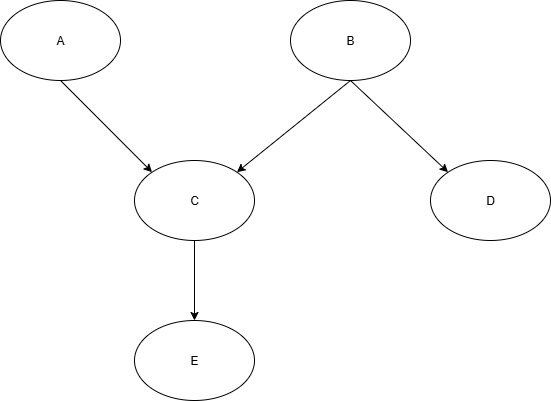
\includegraphics[width=\textwidth]{B_Network_Example.jpg}
		\caption{Example of \acl{bn}}
		\label{fig:bn}
	\end{subfigure}
	\hfill
	\begin{subfigure}[b]{0.45\textwidth}
		\centering
		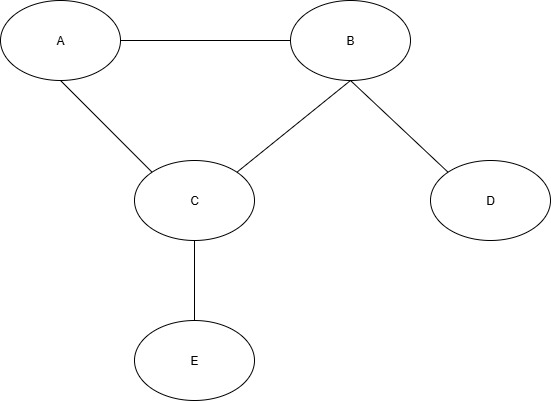
\includegraphics[width=\textwidth]{BN-MN.jpg}
		\caption{Example of \acl{mn} from a \acs{bn}}
		\label{fig:bn-mn}
	\end{subfigure}
	\caption{Conversion of \acl{bn} to \acl{mn}}
	\label{fig:moral}
\end{figure}

Now that all networks are \acs{mn}, the focus shifts to the two main methods of applying inference, \acl{bp} (\acs{bp}) and \acl{bu} (\acs{bu}). These two methods are very similar, with a few differences. 

\acs{bu} is typically applied to a single variable or a small set of variables, using Bayes' Theorem directly: 

\begin{equation}
\text{Posterior belief} = \frac{\text{Likelihood} \times \text{Prior belief}}{\text{Normalization factor}}
\end{equation}

The purpose of \acs{bu} is to refine the belief for a specific variable when new evidence arrives. This update is applied once per new observation, sequentially.

An example for this is if we looks at Figure~\ref{fig:bn-mn}. If evidence at D is observed, Bayesian Updating can be applied to compute the belief for B first, as B is directly connected to D, then the new belief of B can be used to update the beliefs of A and C, which can be extended as far as needed. 

In terms of mathematically explaining this, let evidence be observed at node $D$, denoted $D=d$. Using Bayesian Updating, we first update the belief for the neighboring node $B$:

\begin{equation}
P(B \mid D=d) = \frac{P(D=d \mid B) \, P(B)}{P(D=d)}
\end{equation}

where the normalization factor is

\begin{equation}
P(D=d) = \sum_B P(D=d \mid B) \, P(B).
\end{equation}


Next, we propagate the updated belief to the neighbors of $B$, namely $A$ and $C$:

\begin{equation}
P(A \mid D=d) = \sum_B P(A \mid B) \, P(B \mid D=d),
\end{equation}


\begin{equation}
P(C \mid D=d) = \sum_B P(C \mid B) \, P(B \mid D=d).
\end{equation}

Finally, the belief at $E$ can be updated via \acs{sum} over $C$:

\begin{equation}
P(E \mid D=d) = \sum_C P(E \mid C) \, P(C \mid D=d).
\end{equation}

This demonstrates sequential Bayesian Updating: starting from the observed evidence and propagating through the network to refine the beliefs of all connected nodes.

The other method is \acs{bp}, which is a message passing algorithm for inference in graphical models. This means that each node sends "messages" between each other about variables they have in common. The nodes then combine these messages into beliefs.

\subsubsection{Gaussian Factors}
For object tracking tasks such as in this project, Gaussian factors are especially useful as they can naturally represent noisy measurements of continuous variables, such as the ball's position across the video frames.
Gaussian factors often refer to factors or potential functions defined by a multivariate Gaussian distribution over a set of \acs{rv}. There are two main ways of describing Gaussian (Normal) distributions 

\begin{enumerate}
	\item Mean-Covariance form:\\
	\begin{equation}
	\mathcal{N}(x; \mu, \Sigma) = \frac{1}{(2\pi)^{n/2} |\Sigma|^{1/2}}\exp\left\{ -\frac{1}{2} (x - \mu)^T \Sigma^{-1} (x - \mu) \right\}
	\end{equation}
	where:
	\begin{itemize}
	\item $x$: Vector of \acs{rv}s
	\item $n$: Length of $x$  
	\item Mean ($\mu$): This is the "center" or average of the data.
	\item Covariance ($\Sigma$): This represents how much the values vary and how the different dimensions move together. A higher covariance on the main diagonal represents a lower confidence and large variance from the mean.
	\end{itemize}
	\item Canonical (Information) form:
	\begin{equation}
	C(x; K, h, g) = \exp\left\{ -\frac{1}{2} x^T K x + h^T x + g \right\}
	\end{equation}
	where:
	\begin{itemize}
	\item Information (Precision) Matrix $K$: Inverse of covariance, therefore a higher precision means lower uncertainty ($K = \Sigma^{-1}$)
	\item Information Vector $h$: Related to the mean ($h = K \mu$)
	\item Constant $g$: Adjusts the overall height but isn't always required.
	\end{itemize}
\end{enumerate}

The reason the canonical form is important for using Gaussian factors in a \acs{pgm} is that it allows for more efficient inference. Inference for Gaussian factors in \acs{pgm}s is performed via message passing on a cluster graph, following these steps:

\begin{enumerate}
	\item Create Cluster graph: Group all the factors together into "Clusters" connected by shared variables.
	\item Assign Factors to Clusters: Each cluster's "Potential" is a product of all the Factors assigned to it.
	\item Send messages between Clusters: Each message marginalizes out the cluster's private variables, passing only the shared variables into its neighbor.
	\item Compute Beliefs: Multiply incoming messages at each Cluster to get the final belief over its variables.
\end{enumerate}

\subsubsection{Hybrid Factors}
Hybrid networks are \acs{pgm}s that include both discrete and continuous \acs{rv}s within the same modeling framework. This needs to be discussed because pure discrete networks aren't able to handle continuous measurements, and pure continuous networks can't represent discrete measurements. This section discusses what happens when a network or model has both discrete and continuous \acs{rv}s.

Hybrid factors usually depicted mathematically as:

\begin{equation}\phi(x,y)\end{equation}

where:
\begin{itemize}
	\item $x$: Discrete \acs{rv}s
	\item $y$: Continuous \acs{rv}s
\end{itemize}

What this does is it handles the interaction between categorical decisions and real-valued outcomes. The joint distribution then factorizes as:

\begin{equation}p(x,y) = \prod_{i=1}^{n} \phi_i(X_i, Y_i)\end{equation}

where each factor $\phi_i$ can be either purely discrete, purely continuous or truly hybrid. This factorization is important as it enables inference and represents dependencies.

\paragraph{\acl{clg} (\acs{clg}) Networks}
\mbox{}\\
The most commonly used class of Hybrid Networks is a \acs{clg} network. A \acs{clg} network provides the structure to handle mixed discrete-continuous variables while keeping computational feasibility. A \acs{clg} network is generally preferred over general hybrid models as it is more tractable for inference, allowing for exact probabilistic computation rather than requiring approximation methods.

The \acs{clg} network is a hybrid network where:

\begin{itemize}
	\item Discrete variables can have any parents. (Discrete or Continuous)
	\item Continuous Variables with discrete parents follow a Gaussian distribution whose parameters depend on the parents.
	\item Continuous Variables with continuous parents must follow a linear Gaussian model.
\end{itemize}

\begin{figure}[H]
	\centering
	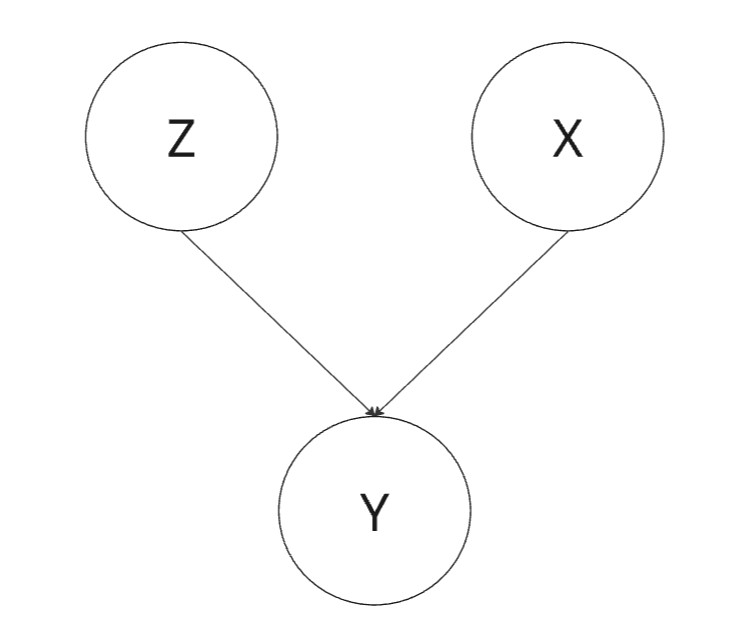
\includegraphics[width=0.4\textwidth]{hybridNet.jpg}
	\caption{Example of a \acl{clg} network showing discrete \acs{rv} $X$ and continuous \acs{rv}s $Y$ and $Z$}
	\label{fig:clg_network}
\end{figure}

A general setup of a \acs{clg} network is shown in Figure~\ref{fig:clg_network}, where $Y$ is a continuous \acs{rv} with discrete parent $X$ and continuous parent $Z$, the conditional distribution is given by:

\begin{equation}P(Y | Z, X=x) = N(Y; \mu_{x}(Z), \Sigma_{x})\end{equation}

where:

\begin{itemize}
	\item $\mu_{x}(Z) = a_{x} + b_{x}Z$ is a linear function of $Z$ with parameters depending on the discrete state $x$.
	\item $\Sigma_{x}$ is the covariance matrix also depending on $x$.
\end{itemize}

With all of this in mind, inference in \acs{clg} networks becomes more complex due to the mixture of discrete and continuous \acs{rv}s. This is where \acl{ep} (\acs{ep}) allows for easier inference.

\subsubsection{\acl{ep} (\acs{ep})}

\acs{ep} is a deterministic approximation technique for \acs{bn}s \parencite{minka2013ep}. \acs{ep} unifies two common approaches to inference techniques, the Kalman filter and Loopy \acs{bp}, which is an extension of previously mentioned \acs{bp} \parencite{minka2013ep}. The method of \acs{ep} is useful for Hybrid networks, as it approximates the belief states by retaining expectations such as means and variances \parencite{minka2013ep}.

\acs{ep} operates by approximating the posterior distribution through iterative moment matching between 'cavity' distributions (approximations excluding one factor's influence, denoted \(q_{-i}(x)\)) and 'tilted' distributions (cavity multiplied by the excluded factor, \(q_{-i}(x) \cdot f_i(x)\)). This process minimizes the Kullback-Leibler divergence \parencite{minka2001expectation,heskes2006approximate}.

\acs{ep} uses an iterative approach which in many cases is computationally infeasible. A special case of \acs{ep} is \acl{adf} (\acs{adf}) or commonly called Moment Matching. This method is done by initializing all the approximating factors except the first one to be uniform and then only allowing a single pass\parencite[510]{bishop2006prml}. This is necessary in the cases when data points arrive sequentially and the model must learn from each point and then discard the data before moving on to the next point \parencite[510]{bishop2006prml}.

Key steps for the \acs{adf} algorithm are as follows:

\begin{enumerate}
	\item \textbf{Initialization:} Start with simple approximations for all factors, assuming minimal prior knowledge.
	\item \textbf{Sequential processing:} Calculate the 'cavity' and 'tilted' distributions and then match moments of the 'tilted' distribution to the Gaussian distribution, updating the approximation immediately.
	\item \textbf{Single Pass:} Unlike the full \acs{ep}'s iterations, the \acs{adf} processes each data point once, discards it and then moves on to the next data point.
\end{enumerate}

\subsection{Gaps}
Despite advancements in commercial ball tracking systems and computer vision techniques, significant gaps remain in accessible, real-time solutions for sports analytics. High costs and infrastructure requirements of systems like Hawk-Eye limit their use beyond professional leagues, while open-source alternatives often lack the precision needed for reliable ball trajectory estimation. Additionally, integrating computer vision outputs with probabilistic graphical models for inference in hybrid networks presents challenges, particularly in handling occlusions, fast motion, and sequential data processing. Approximation methods like Expectation Propagation offer potential, but their computational demands and accuracy trade-offs in dynamic environments require further optimization for low-cost, real-time applications.

\newpage
\section{Model Design}
This section highlights the modular architecture, video footage, the role of \acp{pgm}, and the use of image processing algorithms. Figure~\ref{fig:model_overview} illustrates the overall pipeline of the system. The process begins with a sports video containing a ball. This video is passed through multiple image processing algorithms, each producing an independent estimate of the ball’s position. These outputs are then fused using a \acs{pgm}, which produces a final, unified estimate of the ball’s position.

\begin{figure}[H]
	\centering
	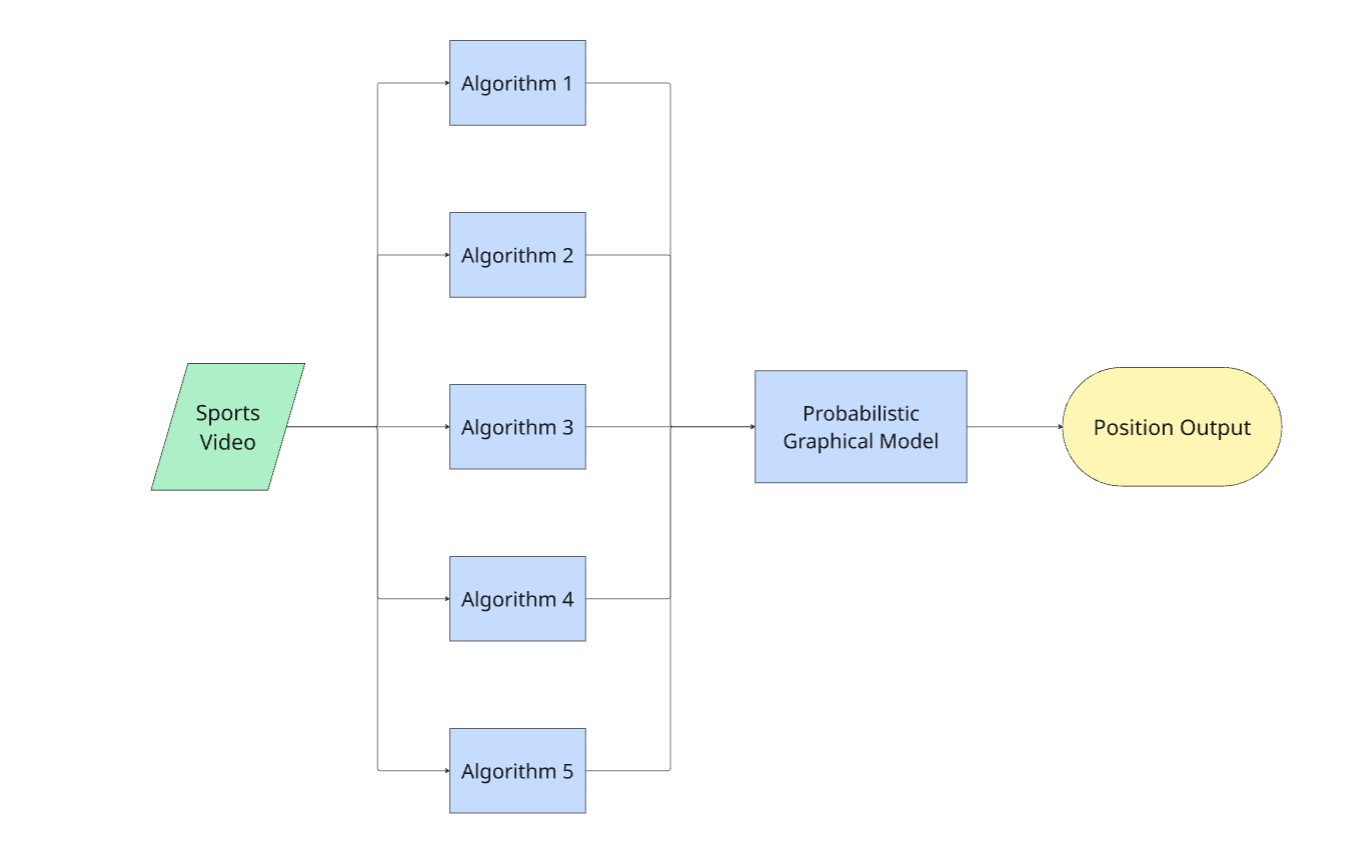
\includegraphics[width=1\textwidth]{ProjectOverview.jpg}
	\caption{Overview of the model design}
	\label{fig:model_overview}
\end{figure}

\subsection{Video Footage Description}

The sports video footage used in this project is sourced from a youtube video that displays a Court Level Tennis practice between Zverev and Djokovic \parencite{youtube_ZverevDjokovic}. The video is 43 minutes long and downloaded in MP4 at 1440p60 quality. The footage is captured at court level, with the camera positioned behind one of the players, where the ball is mostly visible and clearly identifiable. The video will be cut down into shorter video clips where the ball is in play, this is done to ensure manageable processing time, and will be using 30 \acl{fps} (\acs{fps}). The video will be pre-processed to ensure consistent lighting and color balance, which helps improve the performance of the image processing algorithms.

\subsection{\acl{ipa}}
This subsection builds on the discussion of \acs{ipa} in the literature review (Section 2.3), where \acs{ipa}s are categorized into various levels. The purpose of \acs{ipa} in this project is to extract the raw data of the ball's position in each frame of the video and the reason for having multiple \acs{ipa} is to ensure that if one algorithm fails to detect the ball in a frame, the other algorithms and the \acs{pgm} can account for this failure and still provide reliable tracking of the ball. This subsection outlines the requirements needed of the \acs{ipa}, a discussion and design of the various candidate algorithms, and the differences in the algorithms. 

\subsubsection{Requirements}
To ensure that the \acs{ipa}s effectively support ball tracking, they must meet specific requirements. These requirements are derived from the project's needs for real-time performance and robustness to dynamic sports environments, building on the challenges discussed in the literature review. The key requirements for the \acs{ipa}s are outlined in Table~\ref{tab:ipa_requirements}. 

\begin{longtable}{@{} p{0.3\textwidth} p{0.65\textwidth} @{}}
    \caption{Requirements for Image Processing Algorithms}
    \label{tab:ipa_requirements} \\
        \toprule
        \textbf{Requirement} & \textbf{Description} \\
        \midrule
        \endfirsthead
        \toprule
        \textbf{Requirement} & \textbf{Description} \\
        \midrule
        \endhead
        \bottomrule
        \endfoot
        \bottomrule
        \endlastfoot
        Robustness to noise and distractions & The algorithm must reliably track the ball without getting "distracted" by background noise, such as players, lines on the fields or courts, or spectators. This ensures consistent detection in cluttered sports footage. \\
        
        Accuracy in ball center localization & The algorithm should precisely estimate the ball's center position, as well as minimizing errors that could affect trajectory prediction. \\
        
        Process video footage at 30 \acs{fps} & The algorithm must process frames at 30 \acs{fps} to support close to real-time tracking, maintaining efficiency for video analysis without significant time delays. \\
        
        Expand Scalability & The algorithm should handle varying video lengths, resolutions, and input formats with minimal performance degradation, allowing easy adaptation to diverse footage. \\
\end{longtable}

\subsubsection{Algorithm Design}
This subsection discusses the general design of the \acs{ipa}s, to ensure that the requirements in Section 3.2.1 are met. The design is presented as a Flow Diagram as per Figure~\ref{fig:ipaflow}, where the \acs{ipa} needs to be able to take in sports video footage, process each frame, and output an estimated position. The per-frame pixel coordinate $(x,y)$ is normalized by the frame width $W$ and height $H$ as follows:
\begin{equation}
x_{\mathrm{norm}} = \frac{x}{W}, \qquad y_{\mathrm{norm}} = \frac{y}{H}
\end{equation}
which maps positions into the unit square $[0,1]\times[0,1]$. The idea behind using $[-1,-1]$ is that the later \acs{pgm} will be able to identify easily that this input is not ideal and will ignore it since that specific algorithm didn't detect anything in that frame. These outputs then need to be outputted into a text file that can be used in the \acs{pgm}, where the naming of the text file will be \texttt{alg\_n.txt}, where $n \in \{1,...,N\}$ and $N$ is the number of algorithms used. Designing the general \acs{ipa} to work in this way satisfies several of the reqirements, being that it can process each frame at 30 \acs{fps}, it can easily be scaled to various video lengths, and it can be adapted to different video formats. The rest of the requirements will be met according to the specific Low-Level and Intermediate-Level operations used in each algorithm, the position of which can be seen in Figure~\ref{fig:ipaflow}.

\begin{figure}[H]
	\centering
	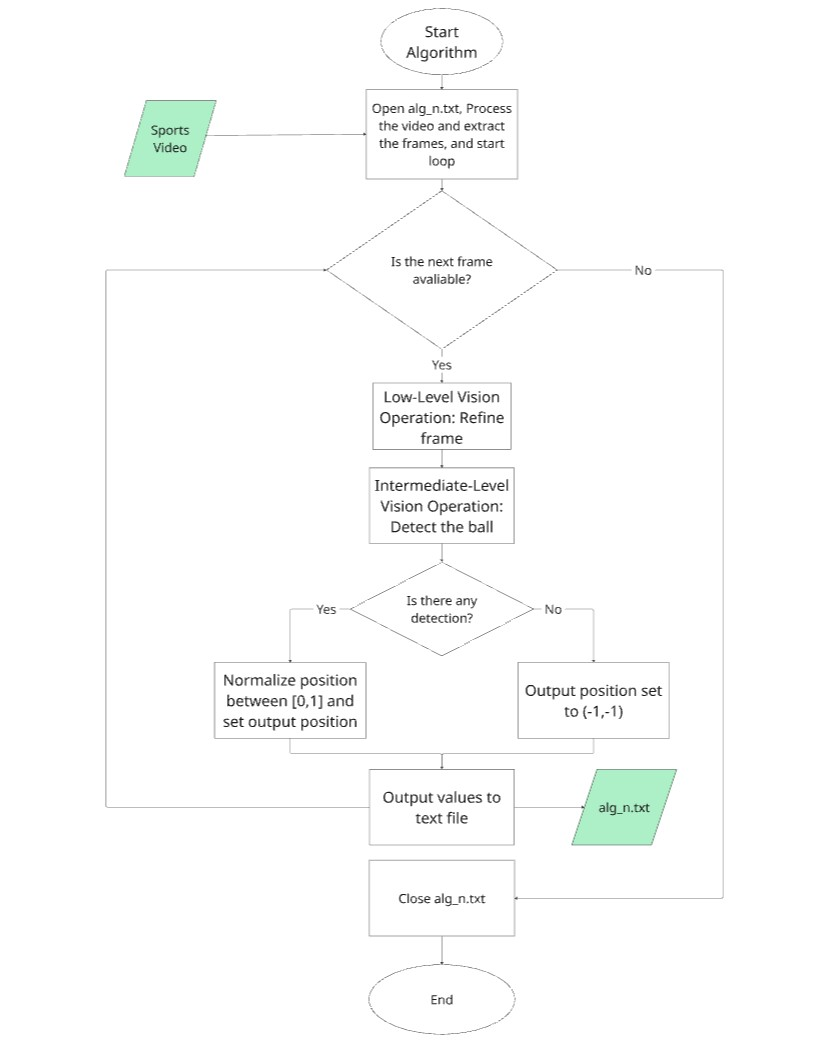
\includegraphics[width=\textwidth]{ipa_flow.jpg}
	\caption{Flow diagram showing the flow of logic each of the \acs{ipa} will follow}
	\label{fig:ipaflow}
\end{figure}

\subsubsection{Candidate Algorithms}
This subsection discusses and guides the design of the various candidate algorithms that can be considered for this project. The functions and operations of these algorithms are based on the OpenCV library, as discussed in Section 2.3.4. The aim of this subsection is to provide various combinations of operations that can be used to create different algorithms, which will then be tested and evaluated to determine the best performing algorithms for this project. The candidate algorithms are summarized in Table~\ref{tab:candidate_algorithms}.

\footnotesize
\begin{longtable}{@{} p{0.15\textwidth} p{0.4\textwidth} p{0.4\textwidth} @{}}
\caption{Candidate Image Processing Algorithms}
\label{tab:candidate_algorithms} \\
    \toprule
    \textbf{Algorithm Name} & \textbf{Low-Level Vision Operation Used} & \textbf{Intermediate-Level Vision Operation Used} \\
    \midrule
    \endfirsthead
    \toprule
    \textbf{Algorithm Name} & \textbf{Low-Level Vision Operation Used} & \textbf{Intermediate-Level Vision Operation Used} \\
    \midrule
    \endhead
    \bottomrule
    \endfoot
    \bottomrule
    \endlastfoot
    HSV Color Thresholding & Median blur and morphological operations & Contour detection and shape analysis \\
    
    Shape-Aware Motion Tracker & Frame differencing, thresholding, and morphological operations & Contour detection, ellipse fitting, and shape analysis \\
    
    Brightness Streak Detector & Frame differencing, thresholding, and dilation & Contour detection and shape analysis \\
    
    Motion Blur Hybrid & Frame differencing, thresholding, and morphological operations & Contour detection and shape analysis \\
    
    Background Subtraction Tracker & Morphological operations & Background subtraction (MOG2), contour detection and shape analysis \\
    
    Canny Edge and Hough Circles & Canny edge detection & Hough circle transform \\
    
    Lucas-Kanade Optical Flow & NA & Optical flow computation and feature tracking \\
    
    Template Matching & Template correlation & Localization \\
    \bottomrule
\end{longtable}

The descriptions for each algorithm are as follows:

\begin{itemize}
    \item \textbf{HSV Color Thresholding:} Reduces noise with median blur, enhances with morphological operations (dilate, erode), finds contours, filters for circular shapes based on shape analysis (aspect ratio, solidity, circularity) to detect the ball.
    
    \item \textbf{Shape-Aware Motion Tracker:} Computes frame differencing, thresholding, morphological operations, detects contours, fits ellipses, applies shape analysis to filter candidates.
    
    \item \textbf{Brightness Streak Detector:} Generates frame differencing, thresholding, dilation, finds contours, applies shape analysis (area, aspect ratio, solidity, circularity).
    
    \item \textbf{Motion Blur Hybrid:} Creates frame differencing, thresholding, morphological operations, detects contours, applies shape analysis for elongated shapes.
    
    \item \textbf{Background Subtraction Tracker:} Applies morphological operations, uses background subtraction (MOG2), detects contours, applies shape analysis (aspect ratio, solidity, circularity).
    
    \item \textbf{Canny Edge + Hough Circles:} Applies Canny edge detection, uses Hough circle transform to detect circles.
    
    \item \textbf{Lucas-Kanade Optical Flow:} Computes optical flow, applies feature tracking to estimate ball trajectory.
    
    \item \textbf{Template Matching:} Uses template correlation for localization of the ball.
\end{itemize}

\subsection{\acl{pgm}}
The purpose of incorporating \acp{pgm} in this project is to combine the outputs of multiple image processing algorithms in a principled and probabilistic manner. These algorithms, while effective individually, are not always reliable, they may occasionally fail to detect the ball or produce inaccurate estimations due to occlusion, motion blur, illumination variation or other visual disturbances. 

A \acs{pgm} allows for a robust fusion of these imperfect outputs by modeling both observed and latent variables, capturing the uncertainty inherent in each tracker’s prediction. This subsection presents the design and construction of the \acs{pgm} model used in the project, including its design requirements, structure, variable definitions, and how inference will be performed to estimate the ball's true position.

\subsubsection{Design Requirements}
In order to effectively design and implement the \acs{pgm} for this project, a clear set of requirements must be defined. These requirements provide a foundation for understanding how the model should be structured, what functionality it must support, and how the final output should behave. In particular, the requirements address aspects such as uncertainty handling, output quality, and model scalability. Table~\ref{tab:pgm_requirements} outlines the key requirements that the proposed \acs{pgm} must satisfy.

\begin{table}[H]
	\centering
	\caption{Requirements for the Probabilistic Graphical Model}
	\label{tab:pgm_requirements}
	\begin{tabularx}{\textwidth}{@{}l X@{}}
		\toprule
		\textbf{Requirement} & \textbf{Description} \\
		\midrule
		Handle uncertainty & The \acs{pgm} must account for noise or missing data in algorithm outputs by modeling them probabilistically. \\
		
		Fuse multiple image processing algorithms & Must combine several algorithm outputs at each frame into a multivariate normal distribution. \\
		
	    Temporal consistency & The model should account for the smooth, continuous nature of the ball's motion by modeling how its position evolves over time, ensuring that current estimates depend on previous positions.\\
		
		Scalable inference & The model must support efficient inference algorithms that remain computationally feasible as the video length increases or as additional tracking algorithms are integrated. \\
		
		Modular design & The structure should allow easy integration or removal of trackers without changing the core model. \\
		
		Factor structure & The relationships between variables must be clearly defined using Gaussian Distributions. \\[1ex]
		\bottomrule
	\end{tabularx}
\end{table}

\subsubsection{Model Construction}
A \acs{bn} was selected for this project as its strengths lie in its ability to explicitly model the dependencies between variables through the use of directed edges. This is \acs{bn}s strength when compared with \acs{mn} for this project, while both can represent complex dependencies and perform inference under uncertainty \parencite{koller2009pgm}, the causal reasoning of the \acs{bn} works well for this project as the image processing algorithms depend on the actual position of the ball.

\textbf{Random Variables}

There are 2 main \acs{rv} per time step, these are presented in Table~\ref{tab:rvs}. 

\begin{table}[H]
	\centering
	\caption{Random Variables for the Probabilistic Graphical Model}
	\label{tab:rvs}
	\begin{tabularx}{\textwidth}{@{}l l X c@{}}
		\toprule
		\textbf{RV} & \textbf{Symbol} & \textbf{Description} & \textbf{Domain} \\
		\midrule
		Ball position & $Pos_{x,y}$ & Actual position of the ball on the screen in normalized coordinates (x and y values) & $[0, 1] \times [0, 1]$ \\
		Algorithm outputs & $Alg_n$ (for $n=1,...,N$) & Output from the $n$-th image processing algorithm & $[0, 1] \times [0, 1]$ \\
		\bottomrule
	\end{tabularx}
\end{table}

Since each image processing algorithm typically outputs a single (x, y) position estimate, this alone does not provide a probability distribution over possible ball locations. To meet the requirement of a multivariate normal distribution in the model, a Gaussian factor is applied to each algorithm’s output.

This transforms the single point estimate into a probabilistic relationship, centered around the algorithm's prediction with an associated covariance that represents its uncertainty. The resulting domain for each algorithm’s output becomes [0,1]×[0,1], with a continuous distribution that reflects the inherent error or noise in the algorithm's estimate.

\textbf{Relationships}

Now that the \acs{rv}s have been defined, the next step is to define the relationships between them. It is evident that the output of each algorithm directly depends on the actual position of the ball. Therefore, there is a causal relationship between $Pos_{x,y}$ and $Alg_n$, as illustrated in Figure~\ref{fig:smallBN}. This implies that the algorithm outputs are conditionally dependent on the true ball position.

\begin{figure}[H]
	\centering
	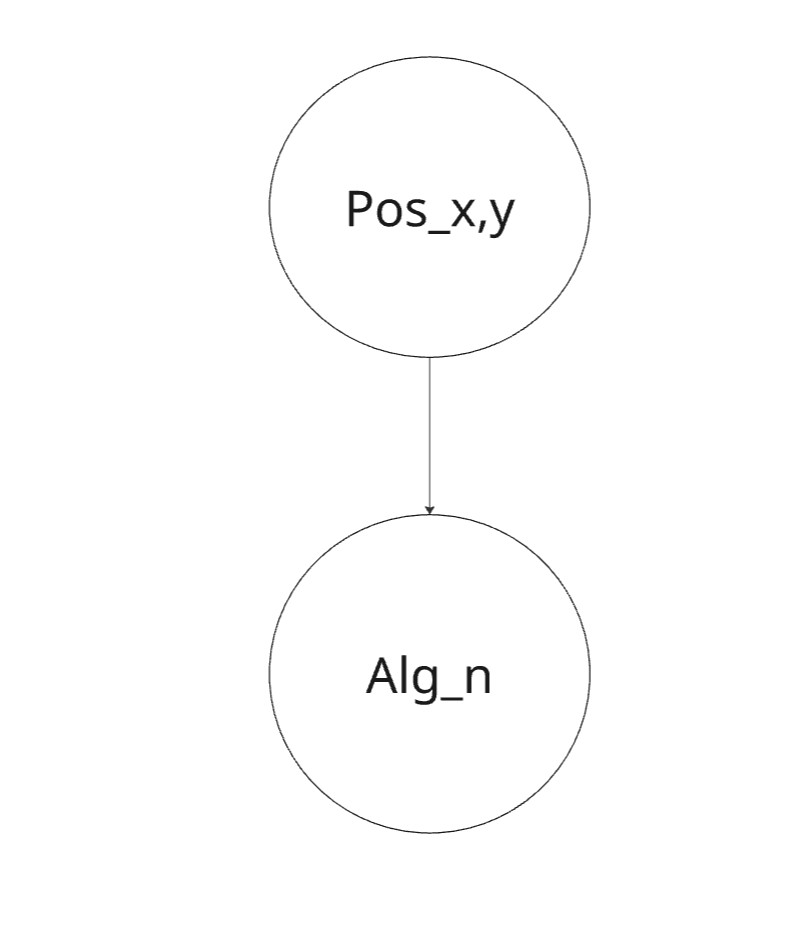
\includegraphics[width=0.25\textwidth]{smallBN.jpg}
	\caption{Relationship between $Pos_{x,y}$ and $Alg_n$}
	\label{fig:smallBN}
\end{figure}

With this in mind, the full model can be defined as shown in Figure~\ref{fig:fullBN}. This represents the final \acs{bn} design used in this project for a single time step. (While the example illustrates five algorithms, the final number is still to be confirmed.)

\begin{figure}[H]
	\centering
	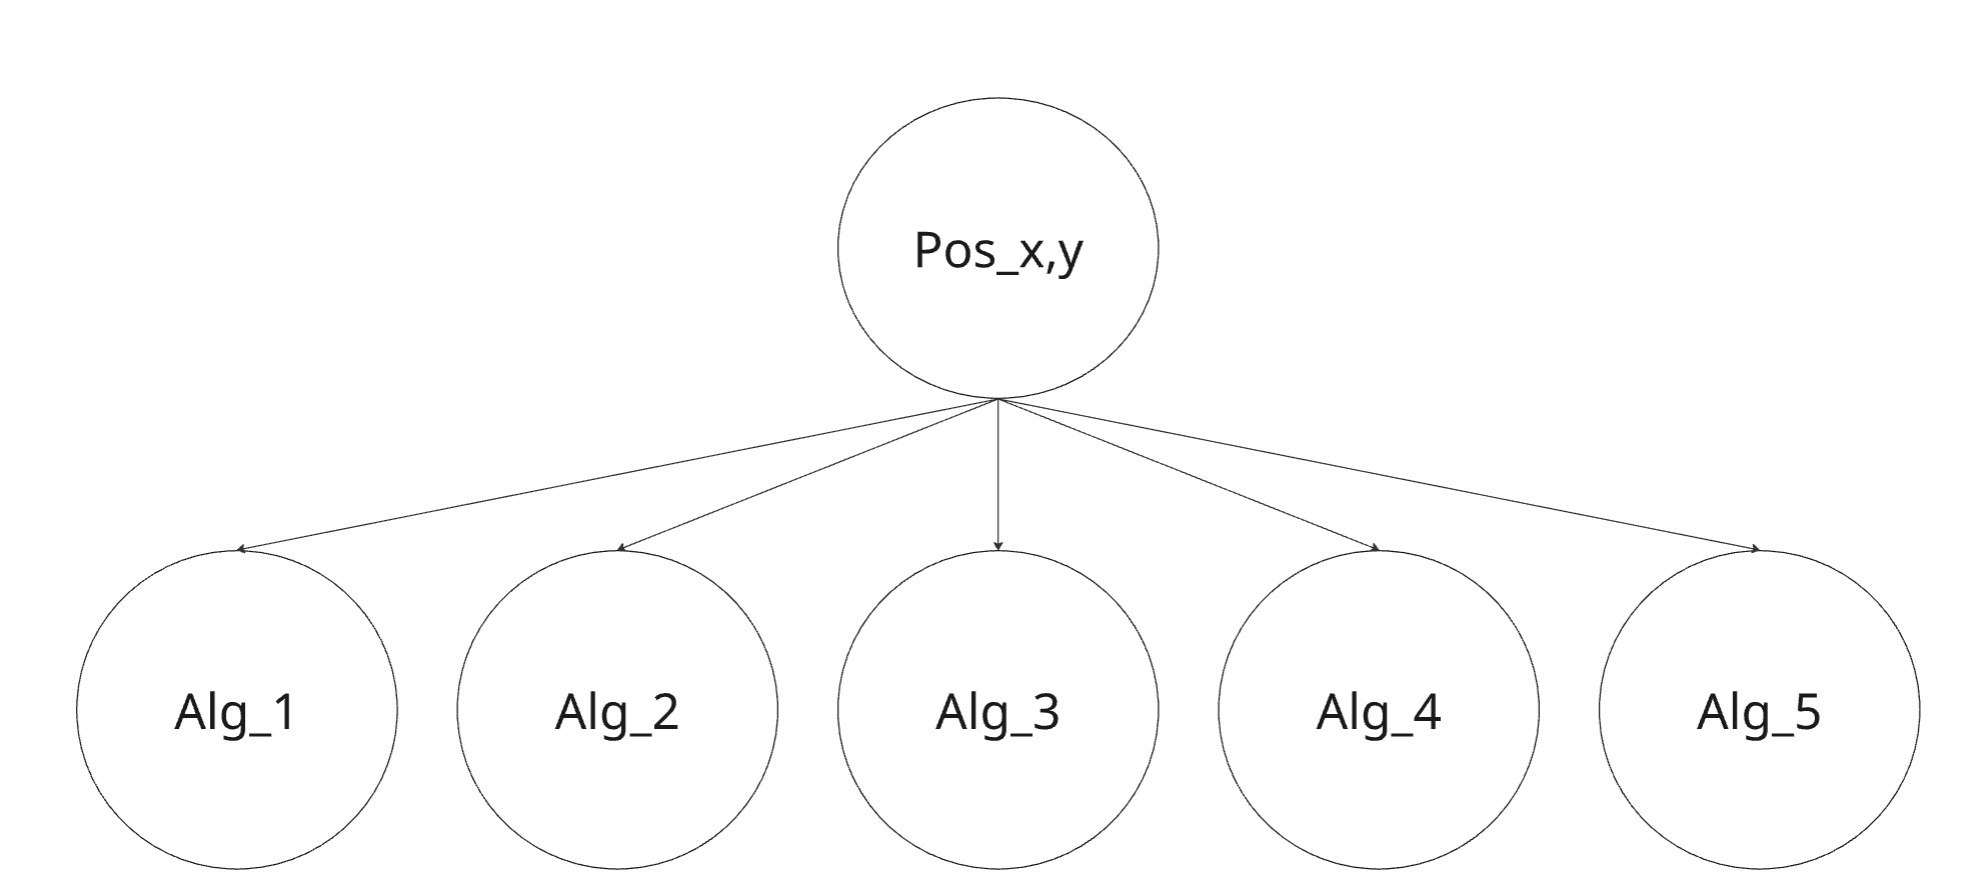
\includegraphics[width=0.6\textwidth]{fullBN.jpg}
	\caption{\acl{bn} showing the relationships between $Pos_{x,y}$ and the various algorithms used}
	\label{fig:fullBN}
\end{figure}


\textbf{Time-step connections}

At this point in order for the ball to be tracked smoothly and efficiently the other frames need to be taken into account. This will be done with $Pos_{x,y}$ having a direct influence on the same \acs{rv} in the next time step. From here the use of $Pos_{x,y}1$, $Pos_{x,y}2$, ..., $Pos_{x,y}n$ will be used per time step. Figure~\ref{fig:fulltimeBN} shows the relationships between each time step. As you can see, $Pos_{x,y}1$ has direct influence on $Pos_{x,y}2$, this means that 
 
 \begin{figure}[H]
 	\centering
 	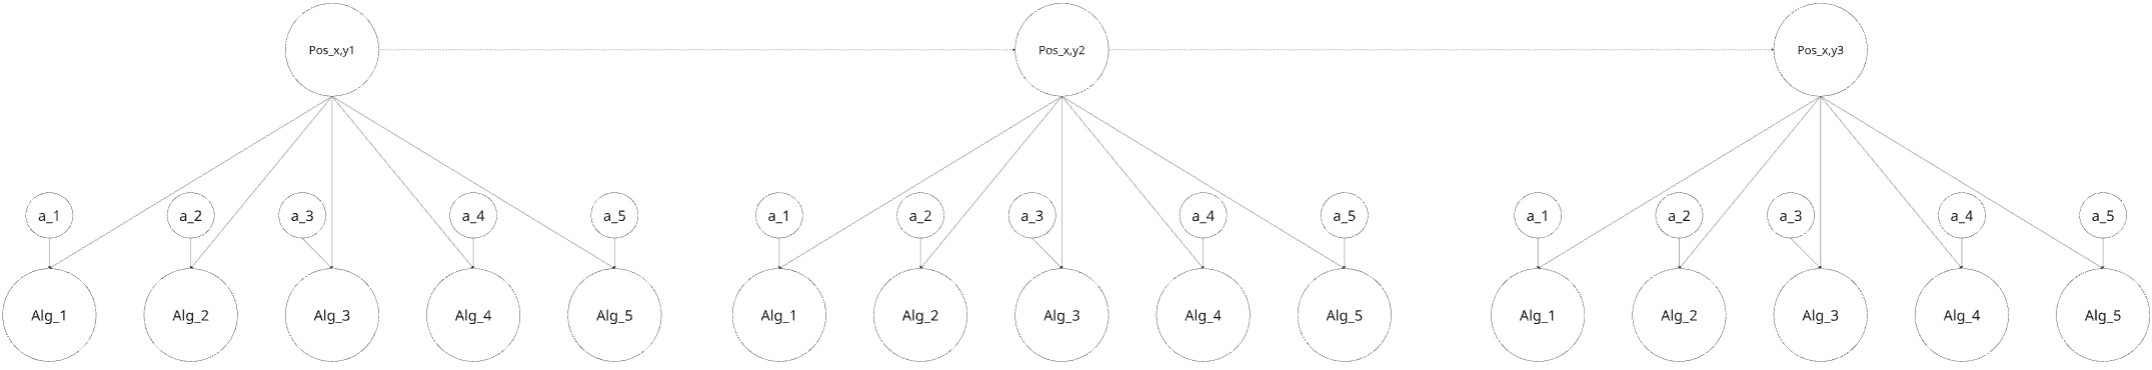
\includegraphics[width=1\textwidth]{BNwtime.jpg}
 	\caption{\acl{bn} showing the relationships between $Pos_{x,y}$ and the various algorithms used at the different time steps}
 	\label{fig:fulltimeBN}
 \end{figure}
 
\subsubsection{Implementing the Model}
This subsection explains how the model will be implemented, detailing both its conceptual workings and the practical coding approach. It will first present the underlying mathematics from first principles, followed by a description of the implementation using the EMDW library developed at Stellenbosch University. (this still needs to be completed, will emphasize more on what was said in the opening paragraph)

\newpage
\section{Still needed to be done}
What still needs to be done is finishing off the lit review, the PGM section and Working on the design of the image processing section. After those are done Testing of the model will be done and the section on testing will be created, this will lead to having to optimize the algorithms used and then finally concluding. Also adding section summaries need to be added per section. Also I need to improve the ECSA table to ensure that they all line up with the sections where I address each of them
\newpage
\printbibliography
\end{document}